%iffalse
\let\negmedspace\undefined
\let\negthickspace\undefined
\documentclass[journal,12pt,twocolumn]{IEEEtran}
\usepackage{cite}
\usepackage{amsmath,amssymb,amsfonts,amsthm}
\usepackage{algorithmic}
\usepackage{graphicx}
\usepackage{textcomp}
\usepackage{xcolor}
\usepackage{txfonts}
\usepackage{listings}
\usepackage{enumitem}
\usepackage{mathtools}
\usepackage{gensymb}
\usepackage{comment}
\usepackage[breaklinks=true]{hyperref}
\usepackage{tkz-euclide} 
\usepackage{listings}
\usepackage{gvv}                                        
%\def\inputGnumericTable{}                                 
\usepackage[latin1]{inputenc}                                
\usepackage{color}                                            
\usepackage{array}                                            
\usepackage{longtable}                                       
\usepackage{calc}                                             
\usepackage{multirow}                                         
\usepackage{hhline}                                           
\usepackage{ifthen}                                           
\usepackage{lscape}
\usepackage{tabularx}
\usepackage{array}
\usepackage{float}


\newtheorem{theorem}{Theorem}[section]
\newtheorem{problem}{Problem}
\newtheorem{proposition}{Proposition}[section]
\newtheorem{lemma}{Lemma}[section]
\newtheorem{corollary}[theorem]{Corollary}
\newtheorem{example}{Example}[section]
\newtheorem{definition}[problem]{Definition}
\newcommand{\BEQA}{\begin{eqnarray}}
\newcommand{\EEQA}{\end{eqnarray}}
\newcommand{\define}{\stackrel{\triangle}{=}}
\theoremstyle{remark}
\newtheorem{rem}{Remark}
\begin{document}

\bibliographystyle{IEEEtran}
\vspace{3cm}

\title{Question 23, CH Gate 2022}
\author{EE23BTECH11017 - Eachempati Mihir Divyansh$^{*}$}
\maketitle
\newpage
\bigskip

\renewcommand{\thefigure}{\theenumi}
\renewcommand{\thetable}{\theenumi}
\textbf{Question:} 
The appropriate feedforward compensator, $G_{ff}$, in the shown block diagram is \\ \\
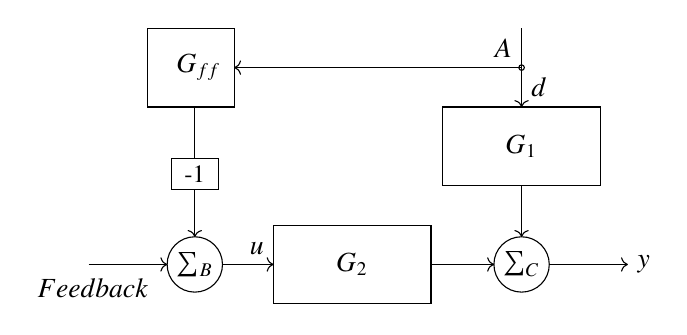
\begin{tikzpicture}
    \draw [->] (-1.35,-5) -- (-0.35, -5); 
    \draw (0,-5) circle (10pt);
    \draw (0,-5) node[]{$\sum_B$};
    \draw [->] (0.35,-5)->(1,-5) node[anchor=south east] {$u$}; 
    \draw (1,-5.5) rectangle (3,-4.5);
    \draw (2, -5) node[] {$G_2$};
    \draw[->] (3, -5) -- (3.8,-5);
    \draw (4.15,-5) circle (10pt);

    \draw (4.15,-5) node[]{$\sum_C$};
    \draw [->] (4.5, -5) -- (5.5,-5) node[anchor=west] {$y$};
    \draw [->] (4.15,-4) -- (4.15,-4.65);
    \draw [->] (3.15,-3) rectangle (5.15,-4);
    \draw [->] (4.15,-2) -- (4.15,-3) node[anchor= south west] {$d$};
    \draw (4.15, -3.5) node[] {$G_1$};
    \draw [<-] (0.5,-2.5) -- (4.15,-2.5) node[above left] {$A$};
    \draw (4.15,-2.5) circle (1pt);
    \draw (-0.6, -3) rectangle (0.5, -2);
    \draw (0.05,-2.5) node[] {$G_{ff}$};
    \draw [->] (0,-3) -- (0, -4.65); 
    \filldraw [color=white] (-0.1, -3.65) rectangle (0.1, -4.05);
    \draw (-0.3, -3.65) rectangle (0.3, -4.05);
    \draw (0,-3.85) node[] {\small{-1}};
    \draw (-1.3, -5.3) node[] {$Feedback$};
\end{tikzpicture}
% \begin{tikzpicture}
%     \draw [->] (-1.35,-5) -- (-0.35, -5); 
%     \draw (0,-5) circle (10pt);
%     \draw (0,-5) node[]{$\sum_B$};
%     \draw [->] (0.35,-5)->(1,-5) node[anchor=south east] {$u$}; 
%     \draw (1,-5.5) rectangle (3,-4.5);
%     \draw (2, -5) node[] {$G_2$};
%     \draw[->] (3, -5) -- (3.8,-5);
%     \draw (4.15,-5) circle (10pt);

%     \draw (4.15,-5) node[]{$\sum_C$};
%     \draw [->] (4.5, -5) -- (5.5,-5) node[anchor=west] {$y$};
%     \draw [->] (4.15,-4) -- (4.15,-4.65);
%     \draw [->] (3.15,-3) rectangle (5.15,-4);
%     \draw [->] (4.15,-2) -- (4.15,-3) node[anchor= south west] {$d$};
%     \draw (4.15, -3.5) node[] {$G_1$};
%     \draw [<-] (0.5,-2.5) -- (4.15,-2.5) node[above left] {$A$};
%     \draw (4.15,-2.5) circle (1pt);
%     \draw (-0.6, -3) rectangle (0.5, -2);
%     \draw (0.05,-2.5) node[] {$G_{ff}$};
%     \draw [->] (0,-3) -- (0, -4.65); 
%     \filldraw [color=white] (-0.1, -3.65) rectangle (0.1, -4.05);
%     \draw (-0.3, -3.65) rectangle (0.3, -4.05);
%     \draw (0,-3.85) node[] {\small{-1}};
%     \draw (-1.3, -5.3) node[] {$Feedback$};
% \end{tikzpicture}\\

\solution \\
%\fi
\begin{table}[h!]
    \centering
    \begin{tabular}{|m{2cm}|m{2cm}|m{2cm}|}
    \hline
    \textbf{Symbol} & \textbf{Value} & \textbf{Description}\\ [1ex]
    \hline
        $x$ & $x\brak{0}r^4$ & $x\brak{4}$ \\ [1ex]
    \hline
        $y$ & $x\brak{0}r^{10}$ & $x\brak{10}$\\ [1ex]
    \hline
        $z$ & $x\brak{0}r^{16}$ & $x\brak{16}$\\ [1ex]
    \hline
        $r$ & ? & $\frac{x\brak{n}}{x\brak{n-1}}$\\[1ex]
    \hline \vspace{0.1cm}
        $x\brak{0}$ & ? & First term \\[1ex]
    \hline
        $x\brak{n}$ & $x\brak{0}r^nu\brak{n}$ & General Term \\ [1ex]
    \hline
    \end{tabular}

    \caption{Input Parameters}
    \label{Gate22.CH23.tab: 1}
\end{table}
\\
In an ideal system, the output $y$ must be independent of the disturbance $d$. This means, the transfer function $$\frac{Y\brak{s}}{D\brak{s}}=0$$
At B, 
\begin{align}
    U\brak{s}=-Y\brak{s}-G_{ff}\brak{s}D\brak{s} \label{Gate22.CH23.eqn: 1}
\end{align}
At C,
\begin{align}
    Y\brak{s}=G_1\brak{s}D\brak{s}+G_2\brak{s}U\brak{s} \label{Gate22.CH23.eqn: 2}
\end{align}
From \eqref{Gate22.CH23.eqn: 1} and \eqref{Gate22.CH23.eqn: 2},
\begin{align}
    &Y\brak{s}=G_1\brak{s}D\brak{s}+G_2\brak{s}\brak{-Y\brak{s}-G_{ff}\brak{s}D\brak{s}}\\
    \implies& \brak{1+G_2}Y\brak{s}=D\brak{s}\brak{G_1\brak{s}-G_2\brak{s}G_{ff}\brak{s}}\\
    \implies& \frac{Y\brak{s}}{D\brak{s}}=\frac{G_1\brak{s}-G_2\brak{s}G_{ff}\brak{s}}{1+G_2}
\end{align}
For this system to be ideal, and from \tabref{Gate22.CH23.tab: 1} 
\begin{align}
    &\frac{G_1\brak{s}-G_2\brak{s}G_{ff}\brak{s}}{1+G_2}=0\\
    \implies& G_{ff}\brak{s} = \frac{G_1}{G_2}\\
    \implies& G_{ff}\brak{s} = \frac{2}{3}\frac{8s+1}{5s+1}
\end{align}
\end{document}

 
